\chapter{METODOLOGI}
\label{chap:metodologi}

% Ubah bagian-bagian berikut dengan isi dari desain dan implementasi

Proses pengerjaan dilakukan sesuai dengan desain sistem berikut dan implementasinya. Perancangan sistem adalah konsep pembuatan dan perancangan infrastruktur. Implementasi sistem adalah proses pengerjaan yang dilakukan berdasarkan desain sistem yang telah dibuat sebelumnya.

%Section 3.1
\section{Metode yang digunakan}
\label{sec:deskripsisistem}
Pada penelitian ini diintegrasikan teknologi visi komputer dengan sistem tertanam agar dapat mengontrol gerak kursi roda menggunakan gerakan mata (\emph{eye gesture}). Gambar \ref{fig:software} merupakan blok diagram \emph{software} yang diimplementasikan dalam penelitian ini.

%Gambar 3.1
\begin{figure} [H] \centering
  % Nama dari file gambar yang diinputkan
  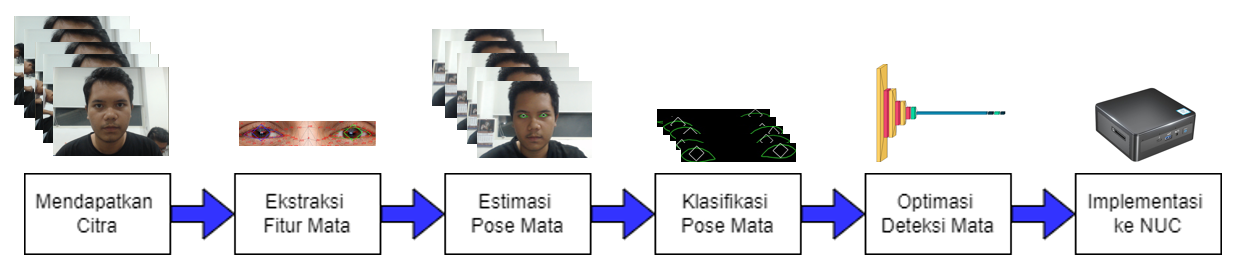
\includegraphics[width=\textwidth]{gambar/bab3/metod.png}
  % Keterangan gambar yang diinputkan
  \caption{Blok Diagram \textit{Software}}
  % Label referensi dari gambar yang diinputkan
  \label{fig:software}
\end{figure}

\subsection{Mendapatkan Citra}

Dalam mengerjakan penelitian ini, langkah pertama yang dilakukan adalah pengambilan citra menggunakan kamera atau sumber gambar lainnya. Citra yang diambil harus cukup jelas dan terfokus pada area wajah agar fitur mata dapat diidentifikasi dengan akurat. Pengambilan citra dapat dilihat pada Gambar \ref{fig:citra}.\\

%Gambar 3.2
\begin{figure} [H] \centering
  % Nama dari file gambar yang diinputkan
  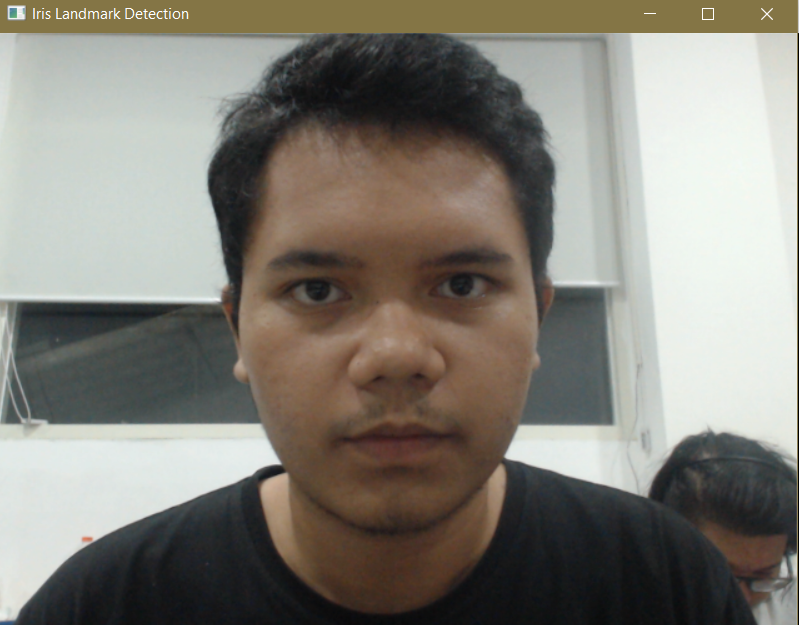
\includegraphics[scale=0.35]{gambar/bab3/citra.png}
  % Keterangan gambar yang diinputkan
  \caption{Pengambilan Citra}
  % Label referensi dari gambar yang diinputkan
  \label{fig:citra}
\end{figure}

\subsection{Ekstraksi Fitur Mata}
Pengenalan pose adalah proses yang melibatkan penggunaan bahasa pemrograman Python, \emph{library} OpenCV, dan \emph{framework} MediaPipe. Dalam konteks ini, Mediapipe berperan penting dalam memperoleh informasi titik \emph{landmark} yang signifikan terhadap objek yang diidentifikasi. \emph{Landmarks} inilah yang menjadi dasar pembentukan representasi visual dari pose tersebut. Proses selanjutnya adalah membuat garis yang menghubungkan titik-titik \emph{landmark} yang diberikan dan menggambarkan hubungan spasial antar titik-titik tersebut. Dengan demikian, metode ini tidak hanya menggunakan Mediapipe Face Mesh sebagai framework utama, tetapi juga  OpenCV sebagai alat analisis gambar dan manipulasi visual yang diperlukan untuk pengenalan pose mata.

Pada penelitian ini akan digunakan salah satu fitur dari MediaPipe yaitu MediaPipe Face Mesh. MediaPipe Face Mesh memiliki cara kerja yang sama dengan MediaPipe, namun MediaPipe Face Mesh secara khusus dibuat untuk mengidentifikasi area wajah manusia. Untuk semua \textit{landmark} yang tersedia pada MediaPipe Face Mesh dapat dilihat pada Gambar \ref{fig:landmark}.

% Gambar 3.3
\begin{figure} [ht] \centering
  % Nama dari file gambar yang diinputkan
  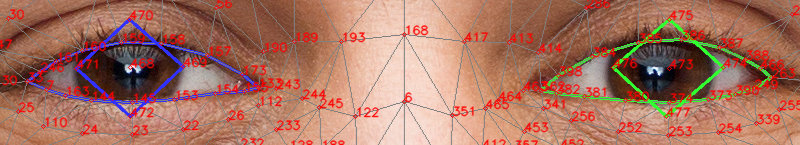
\includegraphics[scale=0.5]{gambar/bab3/landmark2.png}
  % Keterangan gambar yang diinputkan
  \caption{Arsitektur pada MediaPipe Face Mesh \textit{Landmarks}}
  % Label referensi dari gambar yang diinputkan
  \label{fig:landmark}
\end{figure}

Proses pengerjaan penelitian ini akan memanfaatkan teknologi \emph{eye pose detection} dari MediaPipe Face Mesh untuk mengontrol gerak kursi roda. Terdapat beberapa titik yang dibagi menjadi 4 kelas yaitu LEFT\_EYE (kelopak mata sebelah kiri), LEFT\_IRIS (iris mata sebelah kiri), RIGHT\_EYE (kelopak mata sebelah kiri), dan RIGHT\_IRIS (iris mata sebelah kiri). Titik-titik tersebut atau yang disebut dengan \emph{keypoints} akan digunakan pada estimasi pose. Titik-titik \emph{keypoints} yang digunakan pada estimasi pose ini dapat dilihat pada Tabel \ref{tbl:titik keypoints}.

% Tabel 3.1
\begin{table}[H]
\centering
    \caption{Tabel Titik \emph{Keypoints} yang Relevan pada Tahap Estimasi Pose Kelopak Mata dan Iris Mata}
    \label{tbl:titik keypoints}
    \begin{tabular}{|c|c|}                                                                        
     \hline
      Nama        & Keypoints                                                       \\ 
      \hline
      LEFT\_EYE   &362,382,381,380,374,373,390,249,263,466,388,387,386,385,384,398  \\ 
      \hline
      LEFT\_IRIS  &474,475,476,477                                                  \\ 
      \hline
      RIGHT\_EYE  &33,7,163,144,145,153,154,155,133,173,157,158,159,160,161,246    \\ 
      \hline
      RIGHT\_IRIS &469,470,471,472                                                  \\     
      \hline
    \end{tabular}
\end{table}

\subsection{Estimasi Pose Mata}

Proses estimasi pose mata dilakukan dengan mendeteksi keberadaan mata pada citra yang didapatkan. Setelah pose mata didapatkan, selanjutnya dilakukan deteksi untuk 40 titik landmark pada bagian kelopak mata dan iris mata. Untuk melakukan estimasi pose mata, beberapa titik \emph{landmark} yang terdapat pada Tabel \ref{tbl:titik keypoints} akan digambarkan dan diwarnai dengan warna yang unik untuk membantu membedakan setiap bagian mata. Secara spesifik, warna yang diberikan pada setiap titik \emph{landmark} mencerminkan hubungan dengan bagian mata tertentu, sehingga memberikan representasi visual yang detail dan informatif.

Proses ini sangat penting dalam aplikasi pengenalan wajah dan analisis visual, di mana keakuratan dalam mengidentifikasi dan memetakan titik-titik penting pada mata dapat secara signifikan meningkatkan efektivitas sistem. Melalui pendekatan ini, sistem dapat lebih mudah memahami orientasi dan pose mata dalam berbagai kondisi pencahayaan dan sudut pandang, memastikan hasil yang lebih \emph{robust} dan akurat. Untuk lebih jelasnya berikut contoh gambar dengan estimasi pose mata yang dapat dilihat pada Gambar \ref{fig:contoh citra yang telah diestimasi pose} dan Gambar \ref{fig:citratertutup}. 

% Gambar 3.4
\begin{figure} [ht] \centering
    % Nama dari file gambar yang diinputkan
    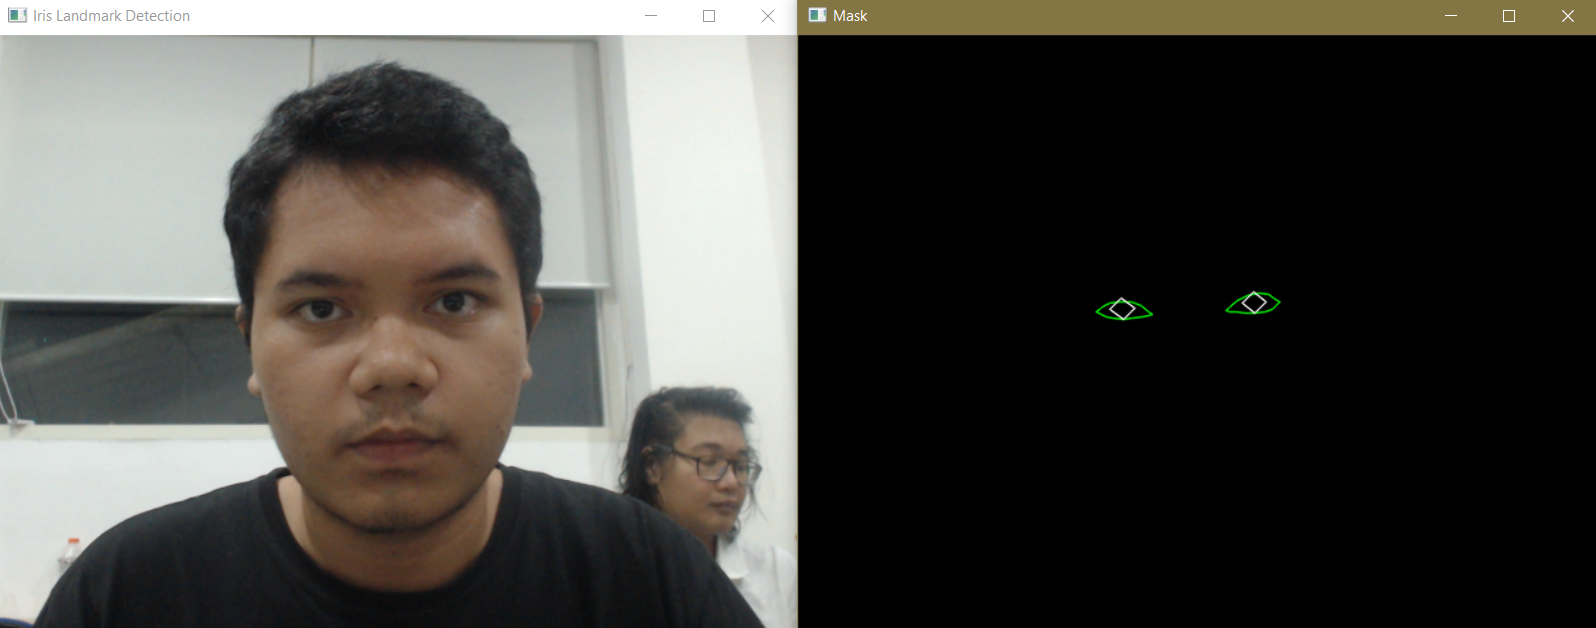
\includegraphics[scale=0.35]{gambar/bab3/iris.png}
    % Keterangan gambar yang diinputkan
    \caption{Citra yang Telah Diestimasi Pose Kelopak Mata dan Iris Mata}
    % Label referensi dari gambar yang diinputkan
    \label{fig:contoh citra yang telah diestimasi pose}
\end{figure}

% Gambar 3.4
\begin{figure} [ht] \centering
  % Nama dari file gambar yang diinputkan
  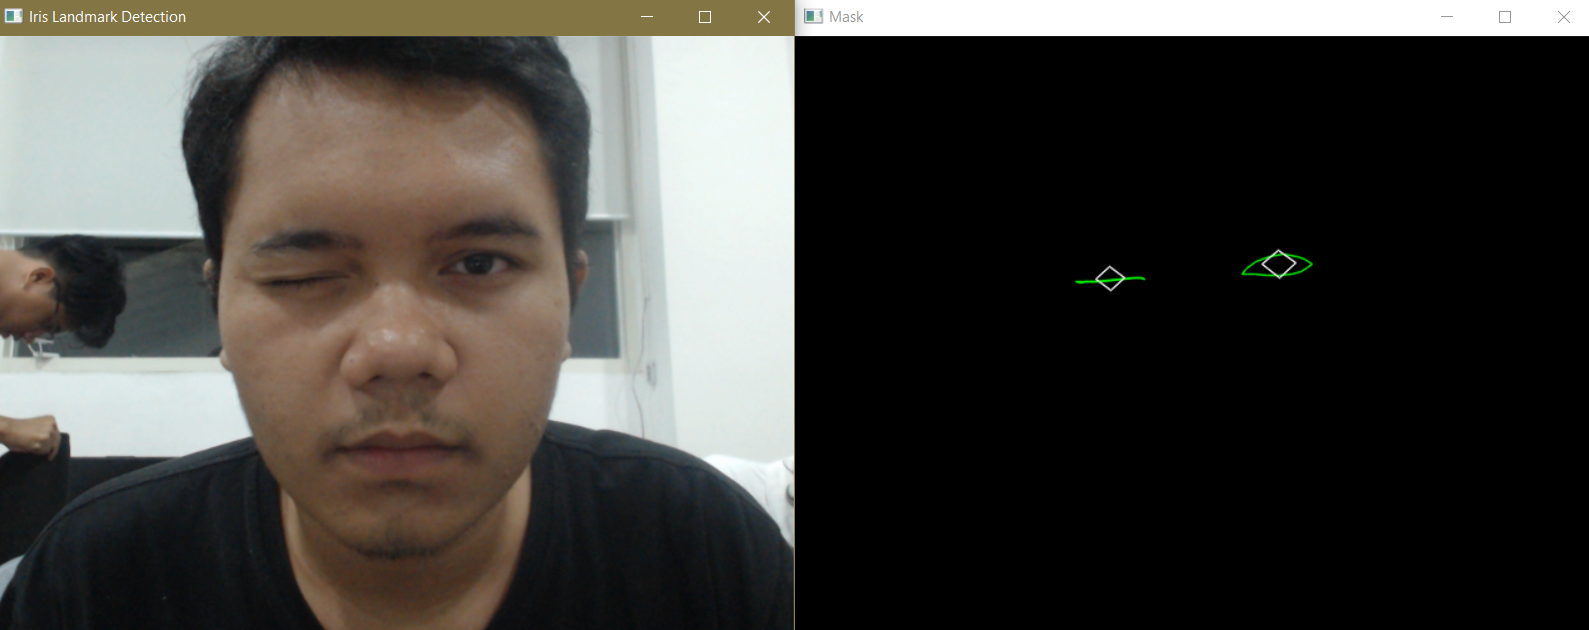
\includegraphics[scale=0.35]{gambar/bab3/stop.png}
  % Keterangan gambar yang diinputkan
  \caption{Citra yang Telah Diestimasi Pose Kelopak Mata Tertutup}
  % Label referensi dari gambar yang diinputkan
  \label{fig:citratertutup}
\end{figure}

\subsection{Klasifikasi Pose Mata}
Setelah proses estimasi pose mata selesai, langkah selanjutnya adalah mengelompokkan citra-citra hasil estimasi ke dalam dataset. Dataset ini akan memiliki 5 kelas berbeda, mewakili perintah untuk bergerak ke kanan, bergerak ke kiri, bergerak maju, bergerak mundur, dan berhenti. 

Pengelompokan ini memungkinkan sistem untuk mempelajari dan memahami pola-pola gerakan mata yang berkaitan dengan masing-masing perintah, sehingga membantu pengembangan algoritma yang dapat secara efektif menerjemahkan isyarat visual menjadi aksi nyata. Dengan demikian, penggunaan dataset yang terstruktur dan terklasifikasi sangat krusial dalam meningkatkan keakuratan respons kursi roda terhadap perintah yang diberikan oleh pengguna.

% Tabel 3.2
\begin{table}[H]
\centering
    \caption{Tabel Contoh Klasifikasi Citra}
    \label{tbl:contoh-klasifikasi}
    \begin{tabular}{|c|c|}
        \hline
        Pose              & Citra              \\ \hline
        Kanan                & 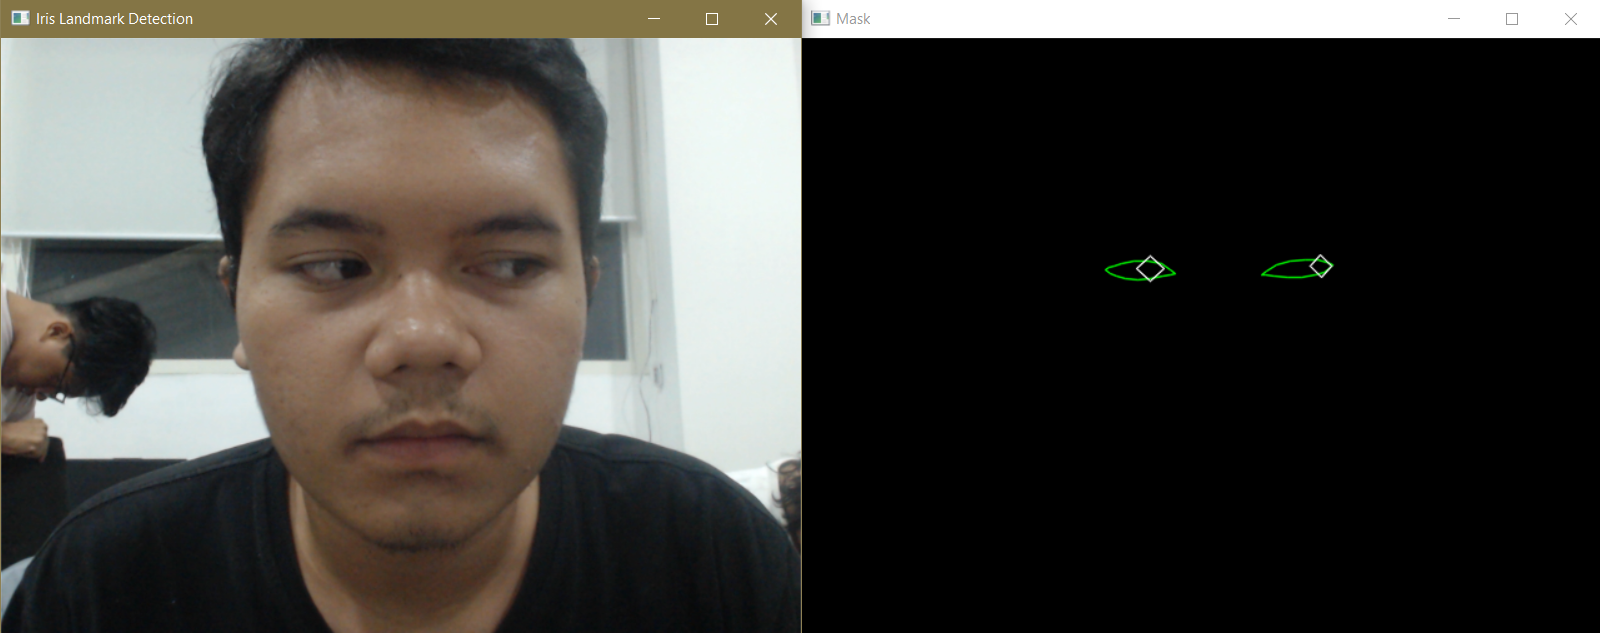
\includegraphics[scale=0.25]{gambar/bab3/kanan.png}   \\ \hline
        Kiri                & 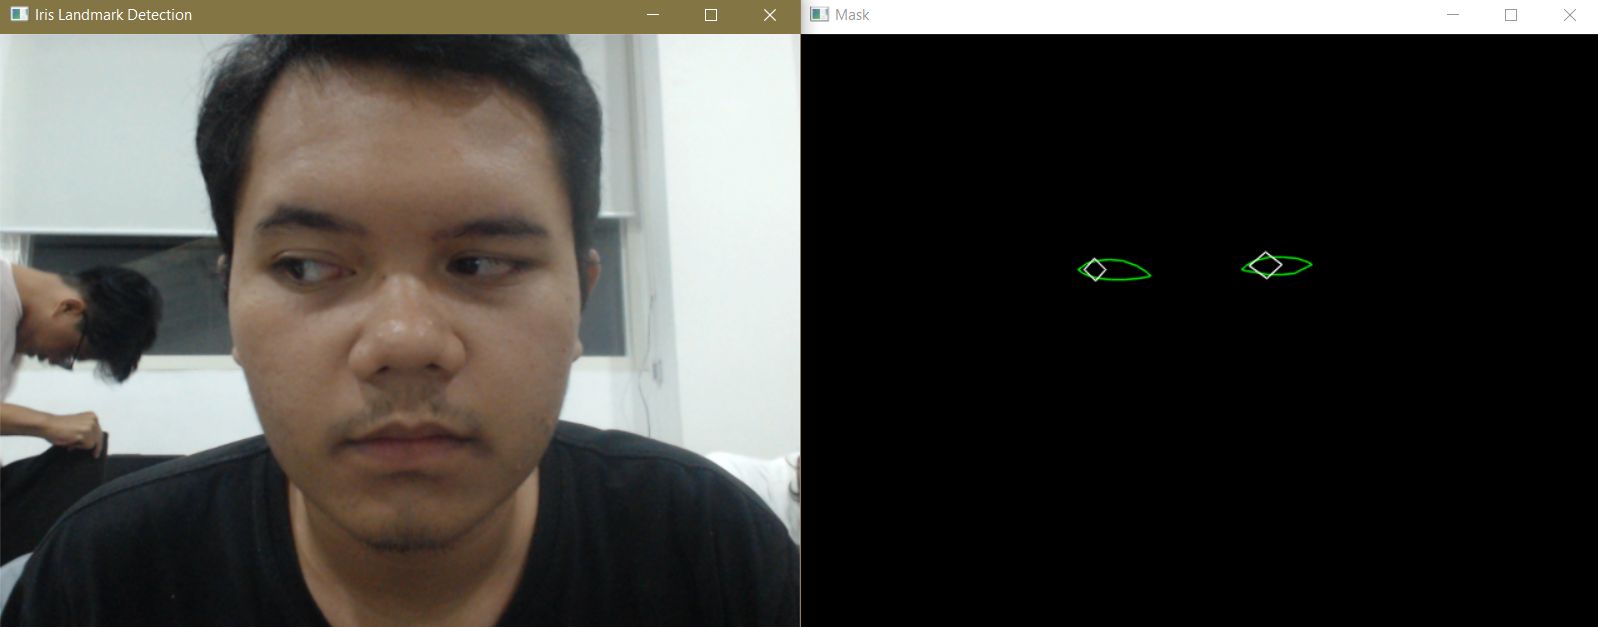
\includegraphics[scale=0.25]{gambar/bab3/kiri.png}   \\ \hline
        Maju               & 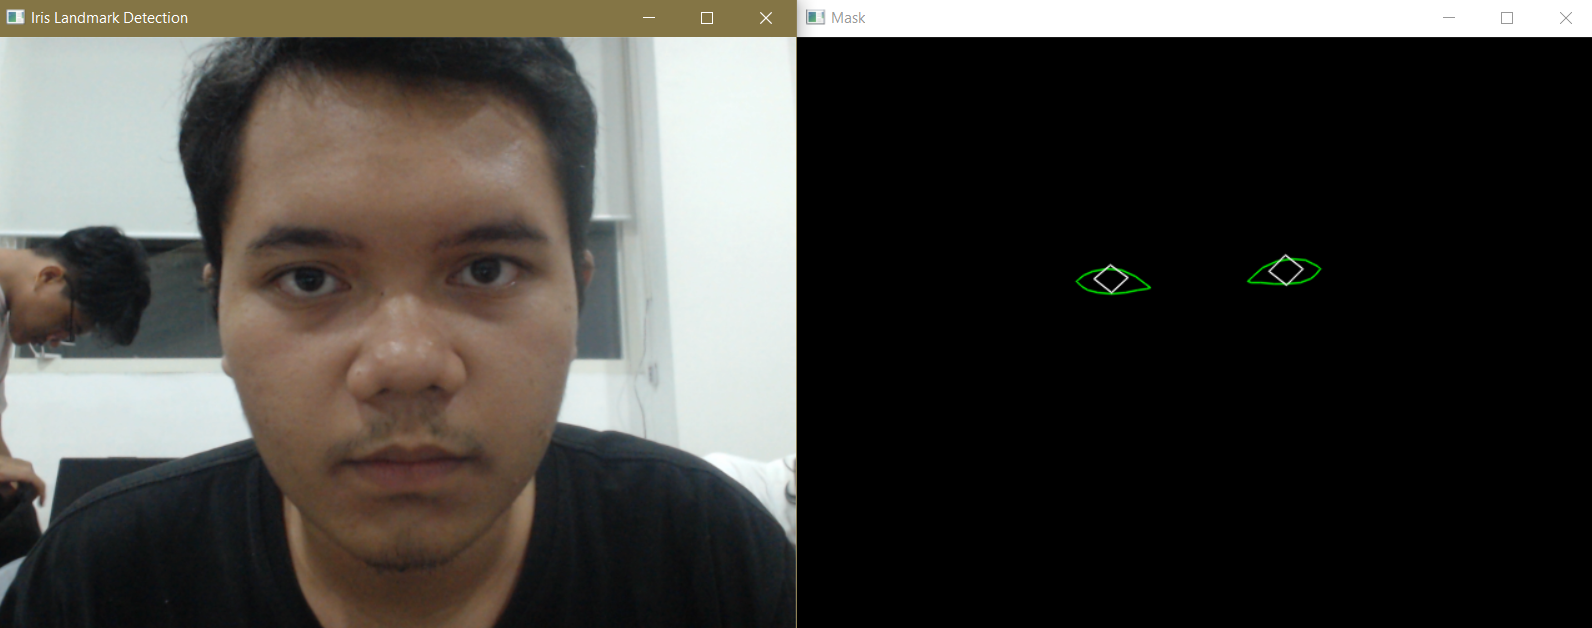
\includegraphics[scale=0.25]{gambar/bab3/maju.png}  \\ \hline
        Mundur               & 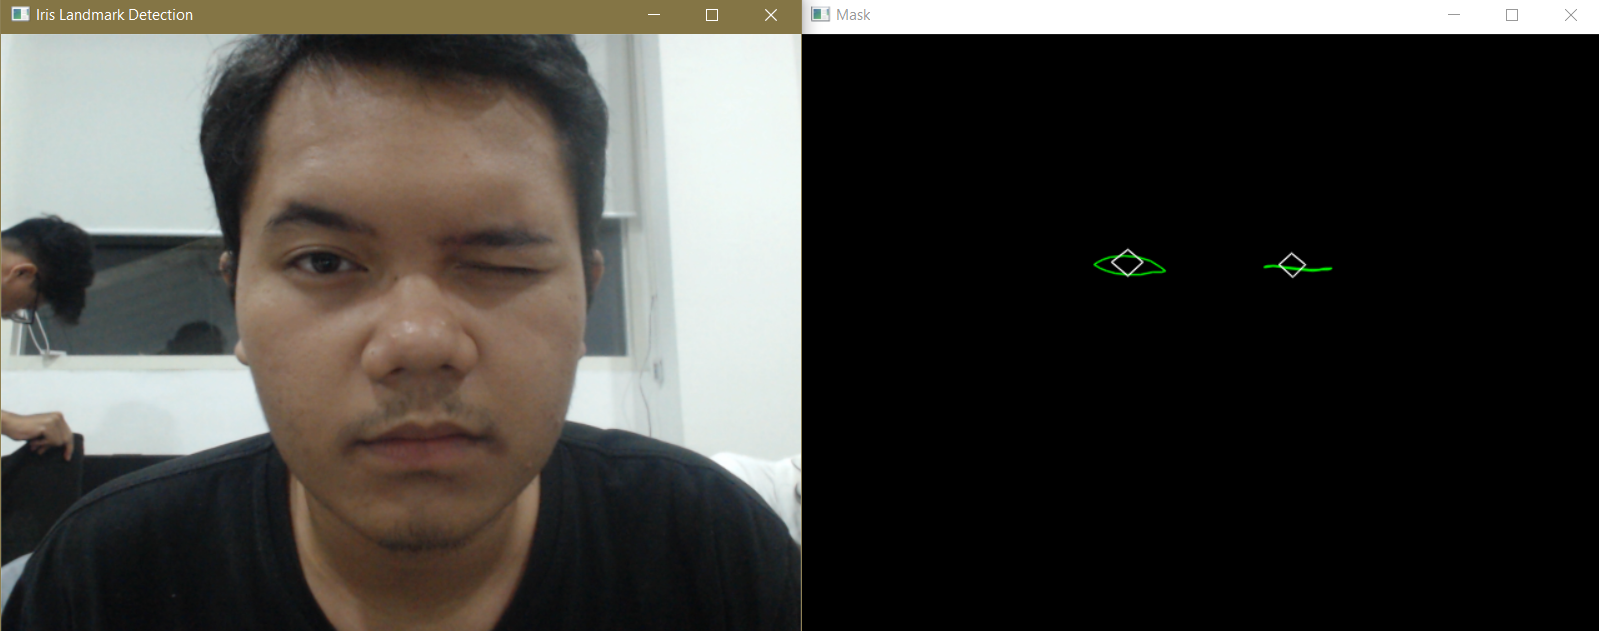
\includegraphics[scale=0.25]{gambar/bab3/mundur.png}  \\ \hline
        Stop               & 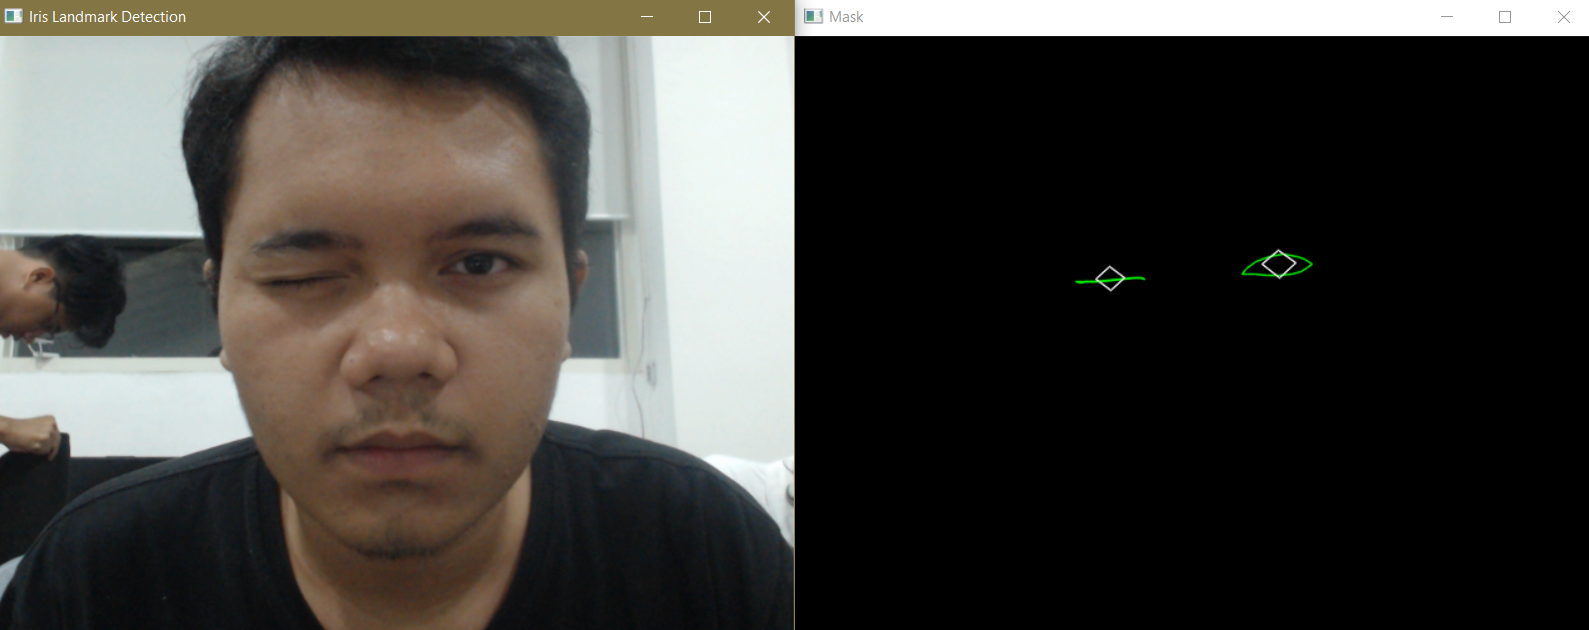
\includegraphics[scale=0.25]{gambar/bab3/stop.png}  \\ \hline
    \end{tabular}
\end{table}

\subsection{Optimasi Deteksi Mata}

Untuk meningkatkan performa dan akurasi, maka dataset melewati proses optimasi menggunakan algoritma \emph{Convolutional Neural Network} (CNN). Langkah ini melibatkan penyesuaian dan peningkatan model CNN untuk meningkatkan akurasi dan efisiensi dalam deteksi mata. Untuk model CNN yang dipakai pada penelitian ini dapat dilihat pada Gambar \ref{fig:layercnn}.

% Gambar 3.5
\begin{figure} [ht] \centering
  % Nama dari file gambar yang diinputkan
  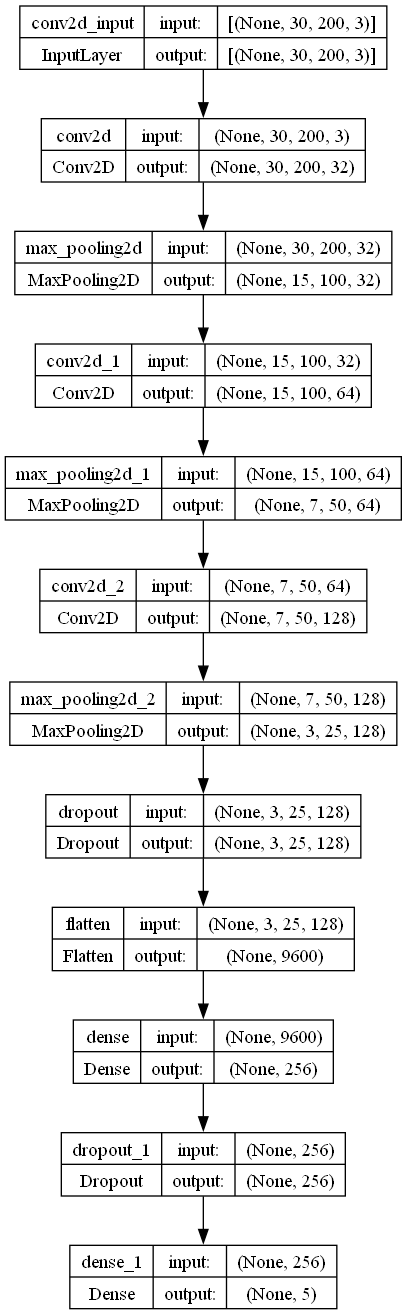
\includegraphics[scale=0.38]{gambar/bab3/layer.png}
  % Keterangan gambar yang diinputkan
  \caption{Visualisasi Layer CNN}
  % Label referensi dari gambar yang diinputkan
  \label{fig:layercnn}
\end{figure}

Gambar di atas menggambarkan arsitektur model jaringan saraf tiruan yang dirancang menggunakan Convolutional Neural Network (CNN). Arsitektur ini dimulai dengan lapisan input yang menerima data gambar berwarna berukuran 30x200 piksel. Kemudian, model dilanjutkan dengan tiga lapisan konvolusi berturut-turut, di mana lapisan konvolusi pertama (Conv2D 1) menggunakan 32 filter dan menghasilkan fitur dengan dimensi `(None, 30, 200, 32)`, lapisan konvolusi kedua (Conv2D 2) menggunakan 64 filter untuk menghasilkan fitur dengan dimensi `(None, 15, 100, 64)`, dan  lapisan konvolusi ketiga (Conv2D 2) menggunakan 64 filter untuk menghasilkan fitur dengan dimensi `(None, 7, 50, 128)`. Setiap lapisan konvolusi ini diikuti oleh lapisan \emph{max pooling} untuk mereduksi dimensi fitur sambil mempertahankan informasi penting, sehingga menghasilkan fitur dengan dimensi `(None, 15, 100, 32)` pada \emph{pooling pertama}, `(None, 7, 50, 64)` pada \emph{pooling kedua}, dan `(None, 3, 25, 128)` pada \emph{pooling} ketiga. Lapisan \emph{dropout} kemudian diterapkan dengan probabilitas 0,25 untuk mencegah \emph{overfitting}.

Selanjutnya, lapisan \emph{flatten} digunakan untuk mengubah tensor hasil konvolusi menjadi vektor datar dengan dimensi `(None, 9600)`. Vektor ini kemudian diteruskan ke lapisan \emph{fully connected} pertama yang memiliki 256 unit neuron, memberikan model kemampuan untuk mempelajari pola-pola kompleks. \emph{Dropout} kembali diterapkan dengan probabilitas 0,5 untuk meningkatkan generalisasi model. Terakhir, lapisan \emph{fully connected} kedua yang juga merupakan lapisan keluaran memiliki 5 unit neuron yang mewakili jumlah kelas target, menghasilkan distribusi probabilitas untuk setiap kelas perintah kontrol gerakan kursi roda seperti "Maju", "Mundur", "Kanan", "Kiri", dan "Stop". Untuk model tiga dimensi layer CNN dapat dilihat pada Gambar \ref{fig:3dlayercnn}.

% Gambar 3.5
\begin{figure} [ht] \centering
  % Nama dari file gambar yang diinputkan
  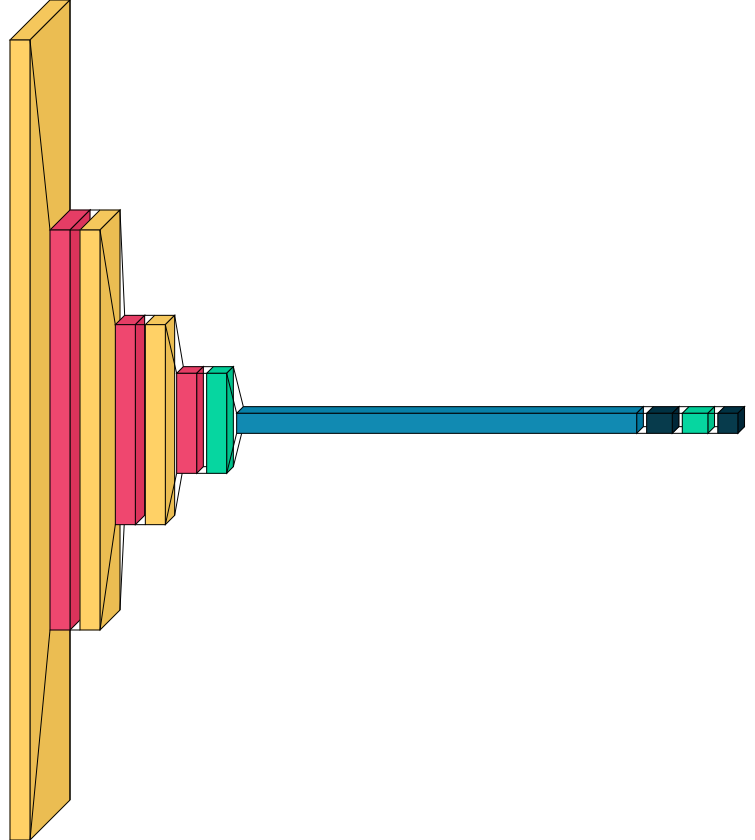
\includegraphics[scale=0.25]{gambar/bab3/3dlayer.png}
  % Keterangan gambar yang diinputkan
  \caption{Visualisasi 3D Layer CNN}
  % Label referensi dari gambar yang diinputkan
  \label{fig:3dlayercnn}
\end{figure}

Sebelum dataset di-\emph{training} menggunakan \emph{layer} CNN, dilakukan beberapa teknik \emph{preprocessing} seperti augmentasi data dan \emph{tuning} parameter. Augmentasi data dilakukan untuk meningkatkan variasi data pelatihan dan mencegah \emph{overfitting}. Teknik augmentasi yang digunakan antara lain \emph{rotation, shearing}, dan \emph{brightness}. Selain augmentasi, \emph{tuning} parameter juga merupakan bagian penting dalam proses ini. \emph{Tuning} parameter melibatkan pengaturan \emph{hyperparameter} model seperti jumlah lapisan konvolusi, ukuran filter, ukuran kernel pooling, tingkat \emph{dropout}, dan ukuran \emph{batch}. Ditambahkan juga beberapa \emph{callbacks} yaitu \emph{rlrop} dan \emph{early stop}. Proses ini bertujuan untuk menemukan kombinasi parameter yang optimal sehingga model dapat dilatih secara efisien dan akurat.

Selain itu, semua gambar dinormalisasi dengan me\emph{rescale}nya ke rentang [0, 1], dengan cara dibagi dengan nilai 265, untuk memastikan bahwa nilai \emph{pixel} konsisten di seluruh dataset. Ini membantu model belajar lebih cepat dan meningkatkan kinerja secara keseluruhan. Dataset kemudian dibagi menjadi tiga bagian: data pelatihan \emph{(training)}, data validasi \emph{(validation)}, dan data pengujian \emph{(testing)}. Pembagian ini memungkinkan model diuji dan divalidasi selama proses pelatihan untuk memantau kinerja secara akurat. Penggunaan CNN dalam optimasi dataset diharapkan dapat menghasilkan model yang mampu mengenali pola dan fitur pose mata dengan akurat, sehingga sistem dapat memberikan respons yang tepat terhadap perubahan perintah yang diberikan oleh pengguna. Spesifikasi perangkat \emph{hardware} yang digunakan untuk \emph{training} dapat dilihat pada Tabel \ref{tb:speklaptop}.

\begin{longtable}{|c|c|c|}
  \caption{Spesifikasi Perangkat Keras}
  \label{tb:speklaptop} \\
  \hline
  \rowcolor[HTML]{C0C0C0}
  \textbf{Perangkat}        & \textbf{Spesifikasi}    \\ \hline
  \multicolumn{1}{|c|}{CPU} & AMD Ryzen 5 4600H       \\ \hline
  \multicolumn{1}{|c|}{GPU} & NVIDIA GeForce GTX 1650 \\ \hline
  RAM                       & 16 GB DDR4              \\ \hline
  Storage                   & 512 GB SSD              \\ \hline
\end{longtable}

Setelah proses \emph{training} selesai, hasil dari model prediksi yang dibuat akan disimpan dalam format h5 (HDF5) untuk memudahkan penyimpanan dan pemuatan. Format ini memungkinkan fleksibilitas dalam menyimpan arsitektur model, bobot, dan konfigurasi lainnya, sehingga memudahkan penggunaan model pada tahap implementasi.

\subsection{Implementasi ke NUC \textit{(Next Unit of Computing)}}

Langkah berikutnya setelah model CNN dioptimasi adalah implementasi model tersebut ke dalam NUC. Ini melibatkan integrasi kode, pengaturan lingkungan runtime, dan pengujian model pada perangkat NUC untuk mengontrol pergerakan kursi roda berbasis gestur mata. Proses ini dimulai dengan integrasi kode untuk menghubungkan model dengan komponen perangkat keras seperti \emph{microcontroller} dan perangkat lunak di NUC. Model CNN yang disimpan dalam format h5 kemudian dimuat, memastikan bahwa model siap digunakan dalam lingkungan NUC.

Selanjutnya, pengaturan lingkungan runtime dilakukan untuk memastikan kompatibilitas antara perangkat keras NUC dan perangkat lunak yang dibutuhkan oleh model. Hal ini mencakup instalasi pustaka seperti TensorFlow, OpenCV, dan pustaka lain yang diperlukan. Pengaturan ini juga memastikan bahwa NUC dapat menjalankan model secara efisien dengan memanfaatkan sumber daya perangkat keras yang tersedia, seperti CPU atau GPU. Tahap berikutnya adalah pengujian model pada perangkat NUC. Pengujian ini melibatkan simulasi perintah gerakan kursi roda berbasis gestur mata. Data gerakan mata yang dikumpulkan melalui kamera diproses oleh model CNN untuk menghasilkan perintah kontrol gerakan seperti "Maju", "Mundur", "Kanan", "Kiri", dan "Stop". Perintah ini kemudian dikirim ke sistem kontrol kursi roda untuk menggerakkan motor sesuai arah yang diinginkan. Selama pengujian, dilakukan pemantauan performa model dalam mendeteksi pose mata dan memberikan respons yang tepat terhadap perintah yang diberikan oleh pengguna.

Selain itu, stabilitas dan kecepatan respons model juga dievaluasi dalam berbagai kondisi pencahayaan dan jarak antara pengguna dengan kamera. Dengan demikian, implementasi ke NUC memastikan bahwa model CNN dapat berfungsi secara real-time dalam mengontrol pergerakan kursi roda berdasarkan pose mata pengguna.

\newpage

%Section 3.2
\section{Bahan dan Peralatan yang Digunakan}

Untuk mendukung penelitian ini, perangkat kontrol yang sudah dikembangkan dibuat agar dapat menerima perintah secara nirkabel dari perangkat lain seperti laptop maupun NUC. Sub bab ini menjelaskan implementasi alat yang dikembangkan dalam penelitian ini.

\subsection{\emph{Hardware} dan \emph{Software} yang Digunakan}
\label{sec:hardware dan software}

Pada penelitian ini, berbagai perangkat keras dan perangkat lunak digunakan untuk membangun sistem kontrol kursi roda berbasis gerakan mata. Berikut adalah daftar perangkat keras dan perangkat lunak yang digunakan:

%List 3.1
\begin{enumerate}[itemsep=0cm] 
    \item Dataset Landmark Pose Mata
    \item Kursi Roda Elektrik
    \item Laptop ASUS TUF Gaming A15 FA506IH\_FX506IH
    \item Kamera Logitech C920
    \item Visual Studio Code
    \item MediaPipe Face Mesh
    \item OpenCV
    \item \textit{Convolutional Neural Network} (CNN)
    \item Intel NUC 11 Pro Performance Kit NUC11PAHi7
    \item ESP32 Devkit V1
    \item Motor Driver H-Bridge
    \item 2 Baterai 24V

\end{enumerate}

\subsection{Alur Kerja Sistem}
\label{sec:alur kerja}

Pada penelitian ini, alur kerja sistem dirancang untuk menjelaskan secara lebih rinci bagaimana perangkat lunak dan perangkat keras berinteraksi dalam mengontrol pergerakan kursi roda menggunakan pose mata. Pertama-tama, kamera menangkap pose mata pengguna dan mengirimkannya ke Intel NUC. Intel NUC kemudian memproses pose ini menggunakan algoritma deteksi pose mata berbasis CNN untuk mengidentifikasi bentuk mata pengguna. Data yang diperoleh dari deteksi pose mata ini kemudian diubah menjadi sinyal perintah untuk menggerakkan kursi roda.

Sinyal perintah yang dihasilkan dari pemrosesan data pose mata dikirim ke \emph{controller} motor kursi roda melalui protokol komunikasi yang sudah ditentukan. \emph{Controller} motor kemudian menerjemahkan sinyal tersebut ke dalam aksi yang sesuai, seperti maju, mundur, berbelok ke kiri, berbelok ke kanan, dan berhenti dengan menggerakkan dan menghentikan motor kursi roda. Seluruh alur kerja ini dijalankan dalam lingkungan perangkat lunak yang dikembangkan menggunakan CNN, OpenCV, dan Mediapipe. Intel NUC berfungsi sebagai pusat kendali yang mengkoordinasikan komunikasi antara berbagai komponen perangkat keras dan perangkat lunak. Dengan integrasi perangkat keras dan perangkat lunak yang baik, sistem ini mampu memberikan respons yang cepat dan akurat terhadap pose mata pengguna.

%Gambar 3.5
\begin{figure} [ht] \centering
  % Nama dari file gambar yang diinputkan
  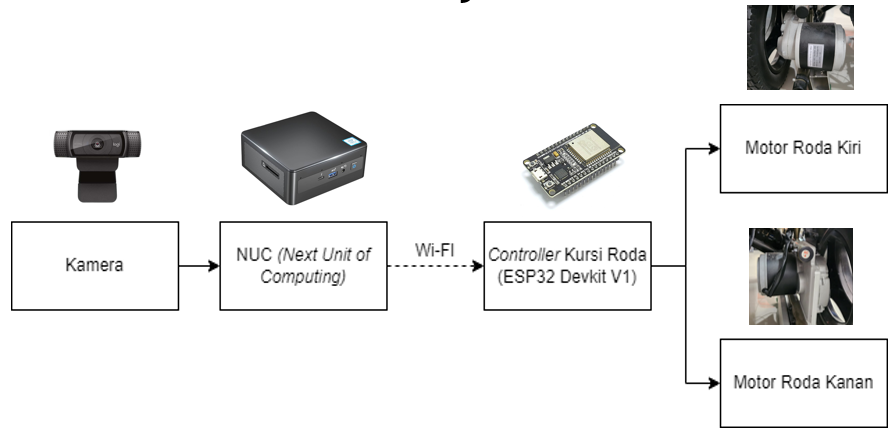
\includegraphics[width=13cm, height=5cm]{gambar/bab3/metod2.png}
  % Keterangan gambar yang diinputkan
  \caption{Blok Diagram \textit{Hardware}}
  % Label referensi dari gambar yang diinputkan
  \label{fig:hardware}
\end{figure}

Gambar \ref{fig:hardware} menggambarkan alur kerja sistem secara keseluruhan. Intel NUC memproses sinyal dari kamera, mengidentifikasi pose mata, dan mengirim perintah ke pengendali motor untuk menggerakkan kursi roda sesuai dengan niat pengguna. Diagram ini memberikan gambaran yang jelas tentang interaksi antara perangkat keras dan perangkat lunak dalam sistem kontrol kursi roda berbasis pose mata ini.

\subsection{Skematik Alat}
\label{sec:skematik}

Skema alat ini dijelaskan secara rinci pada Gambar \ref{fig:Skematik Alat}. Sistem ini memanfaatkan kamera yang terhubung dengan laptop atau NUC sebagai perangkat utama untuk menangkap gambar. Alur kerja dimulai ketika kamera menangkap citra objek, yang kemudian diproses oleh laptop atau NUC. 

%Gambar 3.5
\begin{figure} [H] \centering
  % Nama dari file gambar yang diinputkan
  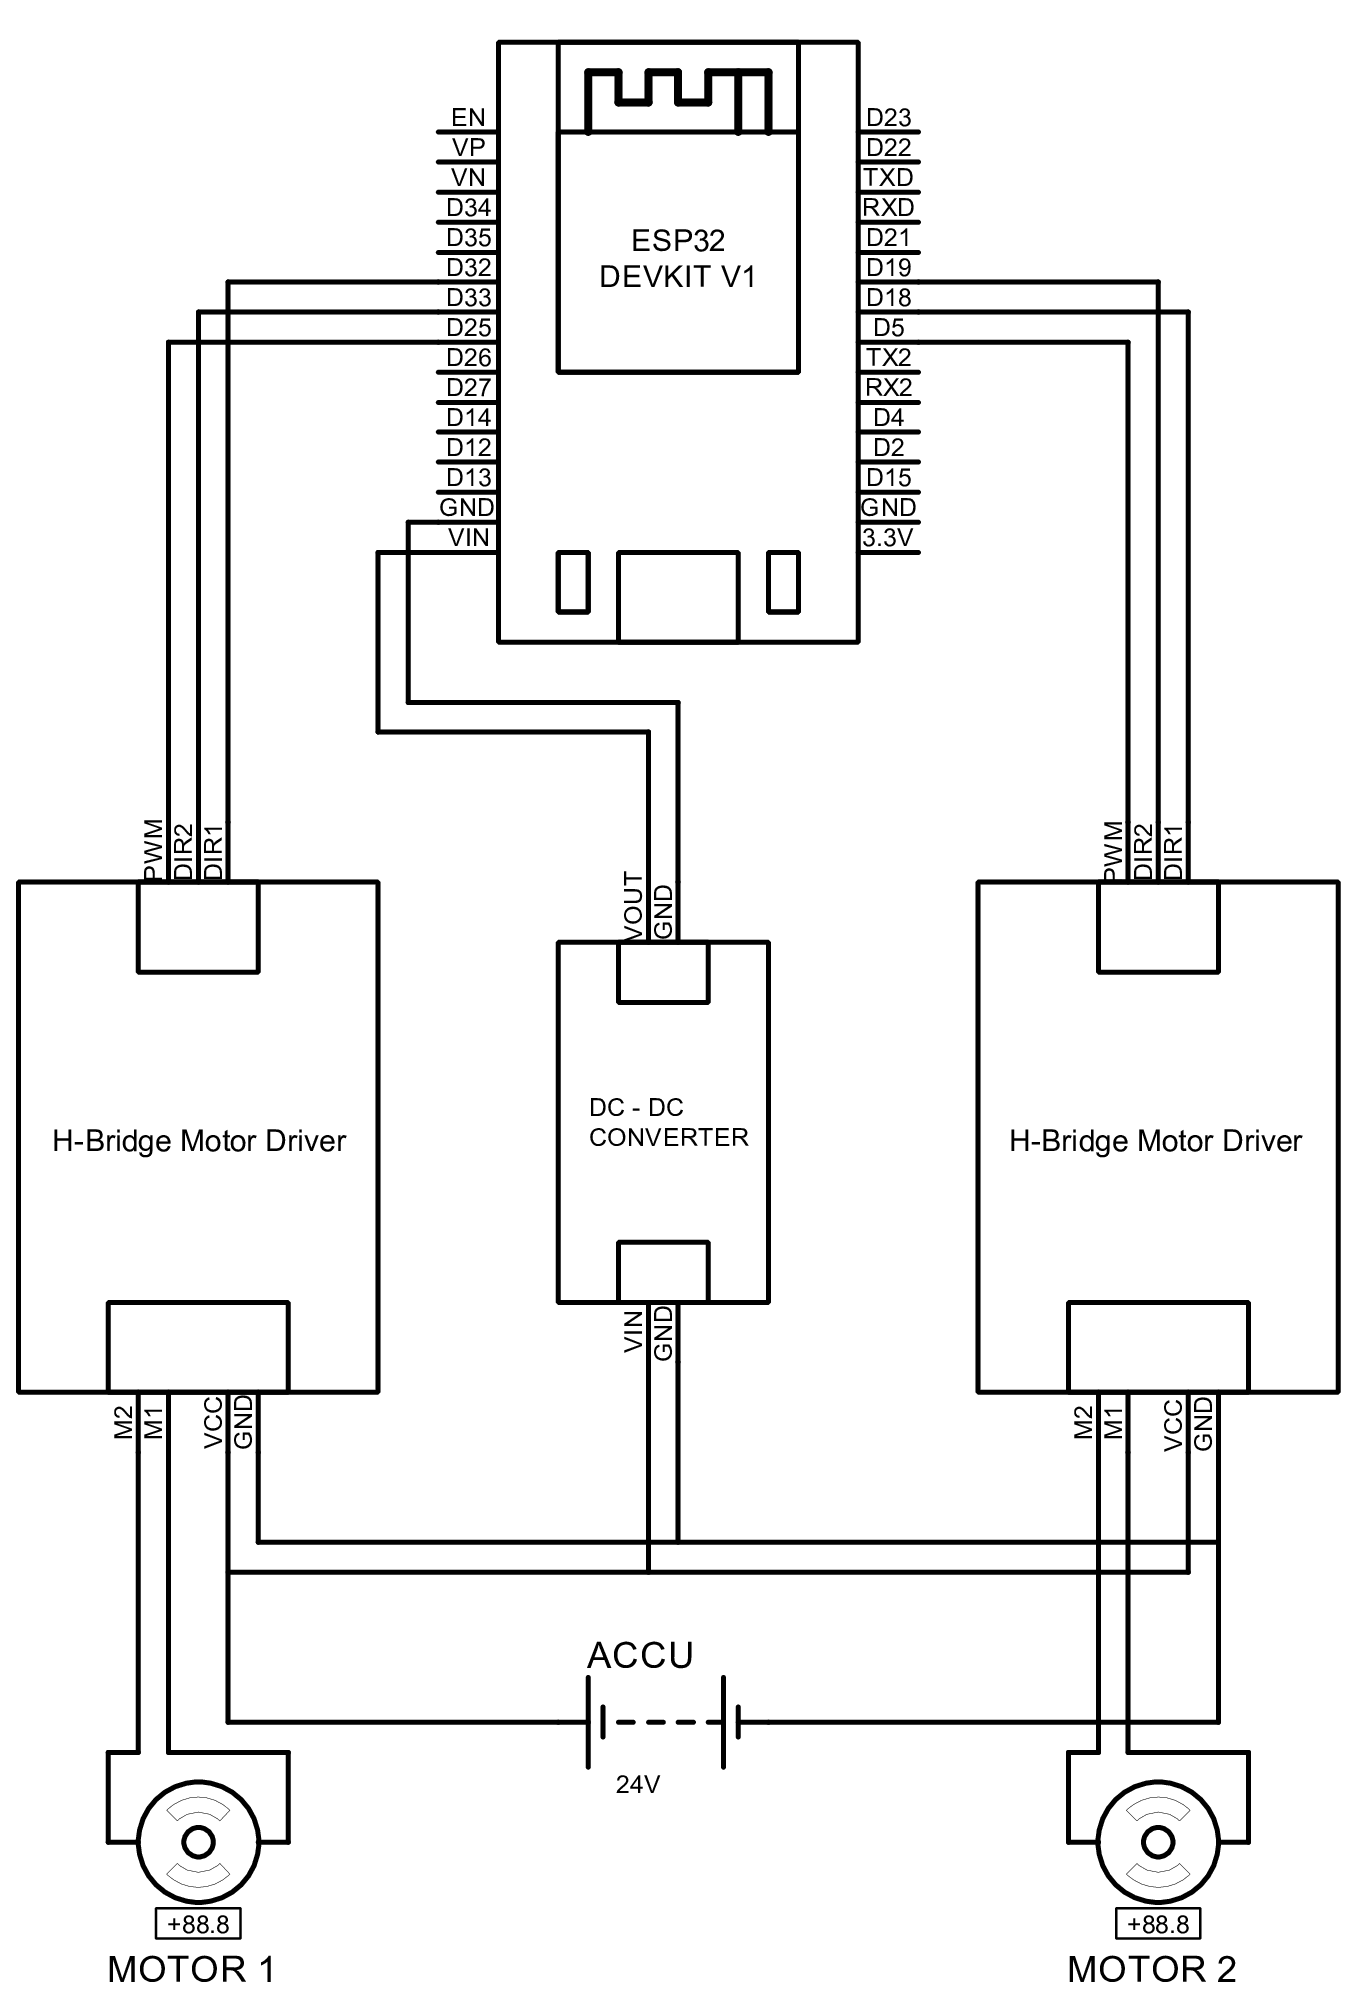
\includegraphics[width=8cm, height=10cm]{gambar/bab3/Schematics.png}
  % Keterangan gambar yang diinputkan
  \caption{Skematik Alat}
  % Label referensi dari gambar yang diinputkan
  \label{fig:Skematik Alat}
  \parencite{ekatama2024perancangan}
\end{figure}

Kode instruksi ini kemudian dikombinasikan dengan parameter kecepatan maksimal yang telah ditetapkan oleh pengguna. Kombinasi antara kode instruksi dan parameter kecepatan ini menjadi satu paket data yang berfungsi untuk mengontrol gerakan kursi roda. Paket data tersebut kemudian ditransmisikan secara nirkabel, baik melalui Bluetooth atau WiFi, ke modul ESP32 Devkit V1.

ESP32 berperan penting dalam mengendalikan motor kursi roda. ESP32 bertindak sebagai pusat kendali yang menerima paket data yang dikirimkan secara nirkabel. Selanjutnya, ESP32 akan memecah paket data tersebut dan menyesuaikannya dengan variabel-variabel yang telah ditentukan sebelumnya. Proses pemecahan paket data ini menghasilkan variabel arah, yang memiliki fungsi penting untuk menentukan arah gerak kedua motor kursi roda. Variabel ini memastikan motor bergerak sesuai arah yang diinginkan berdasarkan data yang diterima \parencite{ekatama2024perancangan}.

\subsection{Mengirim Data String Melalui WiFi}

\emph{Flowchart} ini dirancang untuk mengirim data string ke perangkat ESP32 melalui WiFi. ESP32 akan bertindak sebagai \emph{Access Point}. Berikut merupakan \emph{flowchart} yang digunakan untuk mengirimkan data string melalui WiFi sesuai Gambar \ref{fig:Flowchart 10 Mengirim String WiFi}.

\begin{figure} [H] \centering
  % Nama dari file gambar yang diinputkan
  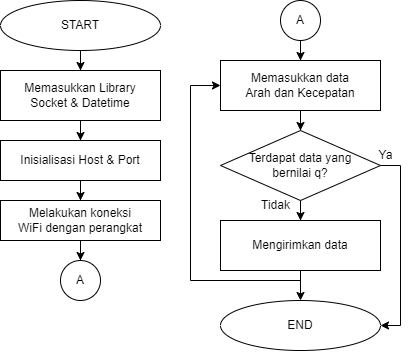
\includegraphics[scale=0.55]{gambar/bab3/10. Mengirim Data String WiFi.png}
  % Keterangan gambar yang diinputkan
  \caption{\emph{Flowchart} Mengirim Data String Melalui WiFi}
  % Label referensi dari gambar yang diinputkan
  \label{fig:Flowchart 10 Mengirim String WiFi}
  \parencite{ekatama2024perancangan}
\end{figure}

Alur kerja program ini menggunakan pustaka \emph{socket}, \emph{time}, dan \emph{datetime}. Pustaka \emph{socket} menyediakan antarmuka untuk membuat dan mengelola soket, sehingga memungkinkan koneksi serta pengiriman dan penerimaan data melalui jaringan. Pustaka \emph{time} menawarkan fungsi-fungsi terkait waktu, seperti \emph{time.sleep()} yang sering digunakan untuk menghentikan sementara eksekusi program selama periode waktu tertentu. Pustaka \emph{datetime} digunakan untuk mendapatkan informasi waktu secara \emph{real-time}.

IP \emph{Address} dari \emph{Access Point} ESP32 kemudian dimasukkan ke dalam variabel \emph{host}, sedangkan nomor port yang digunakan untuk koneksi dimasukkan ke dalam variabel \emph{port}, umumnya port 80. Objek soket dibuat menggunakan \emph{socket.socket()} dengan alamat IPv4 dan tipe soket \emph{streaming}, yang menunjukkan bahwa program ini akan menggunakan protokol TCP/IP untuk koneksi. Program kemudian mencoba terhubung ke server dengan IP \emph{Address} \emph{host} dan nomor \emph{port} yang telah ditentukan.

Setelah koneksi berhasil, program akan berjalan dalam perulangan tak terbatas. Pengguna diminta memasukkan nilai arah dan kecepatan melalui \emph{input}. Nilai-nilai ini kemudian digabung menjadi satu pesan yang dikonversi menjadi \emph{byte} menggunakan \emph{encoding} UTF-8. Setelah dikonversi, pesan tersebut dikirim ke server. Jika pengguna memasukkan "q" sebagai nilai arah atau kecepatan, perulangan akan dihentikan dan program akan menutup koneksi soket \parencite{ekatama2024perancangan}.

\subsection{Menerima Data String Melalui \emph{Access Point} WiFi pada ESP32}

Program ini dirancang sebagai server WiFi yang mampu menerima data dari \emph{client} yang terhubung dan memprosesnya. Program ini memanfaatkan pustaka WiFi untuk mengonfigurasi dan mengelola koneksi WiFi pada ESP32. Variabel \emph{ssid} digunakan untuk menyimpan nama jaringan WiFi yang akan dibuat, sementara variabel \emph{password} menyimpan kata sandi WiFi server. Kedua variabel ini penting agar ESP32 dapat dikonfigurasi sebagai \emph{Access Point}. Kemudian, objek \emph{server} dibuat dari kelas \emph{WiFiServer} untuk menangani koneksi pada port 80.

Di dalam fungsi \emph{void setup()}, \emph{Serial.begin()} digunakan untuk menginisialisasi komunikasi serial dengan kecepatan 115200 bps. Selanjutnya, ESP32 dikonfigurasi sebagai \emph{Access Point} menggunakan SSID dan kata sandi yang telah ditentukan. Setelah \emph{Access Point} berhasil dikonfigurasi, alamat IP ESP32 disimpan dalam variabel \emph{IP} dan ditampilkan di \emph{Serial Monitor}. Fungsi \emph{server.begin()} digunakan untuk memulai server pada port 80.

\begin{figure}[H]
\centering
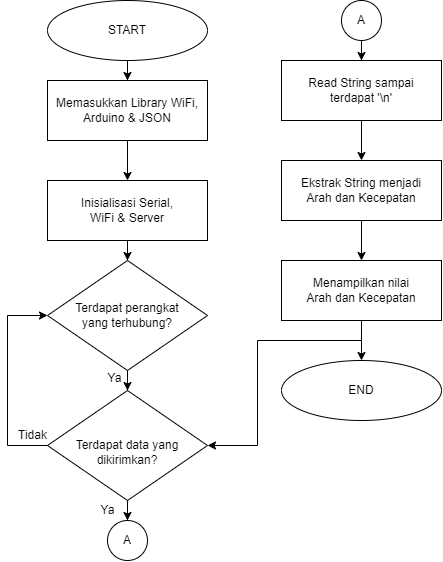
\includegraphics[scale=0.5]{gambar/bab3/4. String WiFi.png}
\caption{\emph{Flowchart} Menerima Data String Melalui \emph{Access Point} WiFi Pada ESP32}
\label{fig:Flowchart 4 String}
\parencite{ekatama2024perancangan}
\end{figure}

Fungsi \emph{void loop()} berjalan terus-menerus setelah \emph{void setup()} dieksekusi. Di dalam fungsi ini, \emph{WiFiClient} digunakan untuk memeriksa apakah ada \emph{client} yang terhubung ke server. Jika ada \emph{client} yang terhubung, program masuk ke dalam blok \emph{if}. Data yang dikirimkan kemudian dibaca secara terus-menerus melalui \emph{while} hingga \emph{client} mengirimkan karakter \emph{newline} ('\textbackslash n'). Nilai variabel ditampilkan di \emph{Serial Monitor} \parencite{ekatama2024perancangan}.

\subsection{Kontrol Motor Kursi Roda Melalui \emph{Access Point} WiFi}

Program ini dirancang untuk mengendalikan motor DC berdasarkan perintah yang diterima melalui koneksi WiFi. ESP32 bertindak sebagai \emph{Access Point}, menerima data arah dan kemudian mengontrol motor kursi roda sesuai dengan instruksi tersebut. Berikut adalah diagram alurnya seperti yang tertera pada Gambar \ref{fig:Flowchart 8 Kontrol WiFi}.

\begin{figure}[H]
\centering
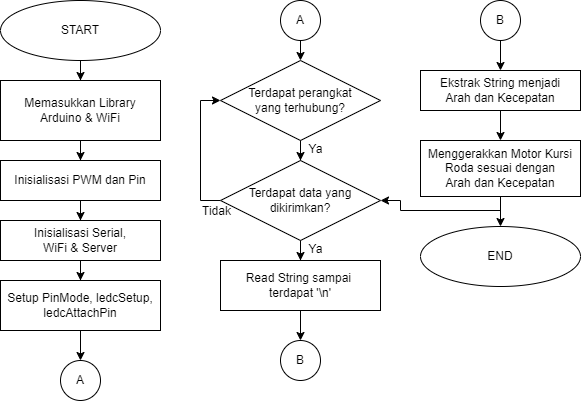
\includegraphics[scale=0.5]{gambar/bab3/8. Kontrol Motor WiFi.png}
\caption{\emph{Flowchart} Kontrol Motor Kursi Roda Melalui \emph{Access Point} WiFi}
\label{fig:Flowchart 8 Kontrol WiFi}
\parencite{ekatama2024perancangan}
\end{figure}

Program ini menggunakan pustaka WiFi untuk mengonfigurasi dan mengelola koneksi WiFi pada ESP32, serta pustaka Arduino untuk fungsi dasar pemrograman mikrokontroler. Variabel \emph{ssid} dan \emph{password} menyimpan nama dan kata sandi untuk \emph{access point} yang dibuat oleh ESP32, sementara objek \emph{server} dari kelas \emph{WiFiServer} menangani koneksi pada port 80. Variabel \emph{pwmpin1, dir1,} dan \emph{dir2} mengendalikan motor kiri, sedangkan \emph{pwmPin2}, \emph{dir3}, dan \emph{dir4} mengendalikan motor kanan. Setiap variabel dihubungkan ke pin GPIO tertentu pada ESP32 untuk kontrol motor. Array \emph{stdir} menyimpan kondisi arah motor, sementara variabel \emph{pwmChannel1, pwmChannel2, freq, res, PWM1\_DutyCycle, maxspeed}, dan \emph{turnspeed} digunakan untuk mengonfigurasi frekuensi dan resolusi PWM, serta kecepatan motor.

Fungsi \emph{void setup()} dijalankan satu kali saat program dimulai. Dalam fungsi ini, \emph{Serial.begin()} menginisialisasi komunikasi serial pada 115200 bps, kemudian \emph{access point} dibuat sesuai SSID dan kata sandi yang ditentukan. IP \emph{Address} ditampilkan pada \emph{Serial Monitor}, dan \emph{server} dimulai pada port 80. Pin kontrol motor diatur sebagai \emph{output}, dan saluran PWM dikonfigurasi dengan \emph{ledcSetup()}. PWM dibagi menjadi 2 kecepatan, yaitu \emph{max speed} dengan nilai sebesar 70 dan \emph{turn speed} dengan nilai sebesar 35.

Pada fungsi \emph{void loop()}, koneksi \emph{client} diperiksa. Jika ada \emph{client} yang terhubung, ESP32 akan membaca data hingga karakter \emph{newline} ('\textbackslash n') dan mengurai data tersebut menjadi variabel arah. Kontrol motor dilakukan menggunakan pernyataan \emph{if-else} berdasarkan nilai variabel arah yang diterima. Setiap kondisi melibatkan perulangan \emph{while} untuk memastikan perubahan kecepatan motor terjadi secara bertahap. \emph{digitalWrite()} menetapkan arah motor, sementara \emph{ledcWrite()} mengendalikan kecepatan motor. Perulangan ini terus berlanjut selama ESP32 menerima data melalui WiFi \parencite{ekatama2024perancangan}.